\chapter{Implementacja}
\label{chap:Implementacja}

W~rozdziale \ref{chap:ProjektSystemu} przedstawiono autorskie
rozwiązanie problemu monitorowania klienta mobilnego przy użyciu
systemu {\em Icinga}. W~ramach projektowania takiego systemu dokonano
analizy dostępnych na rynku dodatków pod kątem ich przydatności
w~systemie monitorowania klienta mobilnego. Przeprowadzona analiza
wykazała konieczność opracowania nowego dodatku, pozwalającego na
przekazywanie w~sposób zgodny z~wymaganiami, danych z~urządzenia
mobilnego do serwera.  Dodatek ten --- NSCAv2 został zaprojektowany
i~zaimplementowany w~ramach niniejszej pracy. Rozdział ten zawiera
dokładny opis funkcjonalny tego dodatku oraz przedstawia istotne
elementy jego implementacji.

Ponadto, w~proponowanym systemie występuje aplikacja przeznaczona dla
platformy mobilnej. Implementacja takiej aplikacji wykracza poza
zakres tej pracy.  W~ramach serii prac dyplomowych przygotowywanych na
Wydziale Elektroniki i~Technik Informacyjnych powstała również praca
inżynierska Pana Marcina Kubika. Przedmiotem tej pracy jest projekt
oraz implementacja dla platformy Android aplikacji
IcingaMini. Pobieżny opis koncepcji i~potrzeby tej aplikacji można
znaleźć w~rozdz.~\ref{sec:IcingaMini} natomiast szczegółowy opis
implementacji został zawarty w~\cite{book:pracaKubika}.

\section[Opis architektury][Opis architektury]{Opis architektury}


Konceptualny model dodatku został przedstawiony
w~rozdz.~\ref{sec:ProjModOdb}. Fizyczna struktura programu jest dużo
bardziej złożona. Została utworzona z~użyciem biblioteki Qt jako
podstawowego szkieletu aplikacji. Wykorzystano również biblioteki
boost oraz Crypto++. Dodatek ten przeznaczony jest, podobnie jak
system monitorujący {\em Icinga}, dla komputerów pracujących pod
kontrolą systemu operacyjnego Linux i~jest uruchamiany jako
samodzielny serwis. Fizyczna struktura programu składa się
z~następujących elementów:

\begin{description}
\item[szkielet programu] --- Zawiera elementy programu konieczne do
  wytworzenia środowiska dla funkcjonowania pozostałych modułów oraz
  zarządzania nimi. Ponadto zawiera odwzorowanie bytów logicznych
  (dostawca, konsument, kanał komunikacyjny) programu w strukturę
  fizyczną.
\item[moduł kryptograficzny] --- Dostarcza implementacji funkcji
  kryptograficznych, wymaganych podczas komunikacji z klientem
  mobilnym. Zawiera zarówno algorytmy asymetryczne, konieczne do
  inicjalizacji kryptografii symetrycznej, jak i~algorytmy
  symetryczne, służące do przesyłania danych.
\item[moduł autoryzacji klienta] --- Zawiera implementację algorytmów
  uwierzytelnienia klienta.
\item[moduł komunikacji z użyciem TCP] --- Dostarcza implementację
  protokołu komunikacyjnego używanego do komunikacji z~klientem.
\item[moduł logowania] --- Pozwala na przekazywanie użytkownikowi
  komunikatów z~dowolnych miejsc znajdujących się w~innych
  modułach. Wiadomość ta może zawierać informacje o~zaistniałym
  błędzie lub innym zdarzeniu, wymagającym poinformowania użytkownika.
\end{description}

Odwzorowanie podstawowych elementów struktury logicznej w~fizyczną ma
miejsce w~szkielecie aplikacji. Pozostałe elementy programu zostały
zaprojektowane jako moduły pomocnicze świadczące dobrze zdefiniowane
usługi. Szczególnym przykładem tego usługowego charakteru pozostałych
modułów może być moduł kryptograficzny i~moduł autoryzacji
klienta. Udostępniają one generyczne interfejsy dostępu do swoich
usług dla pozostałych modułów. Szczegóły implementacyjne są natomiast
zamknięte wewnątrz modułów. Typ faktyczny obiektu udostępnianego
poprzez generyczny interfejs jest w~bardzo wielu przypadkach
determinowany dopiero na etapie konfiguracji programu. Ponadto liczba
klas znajdujących się w~tych modułach może znacząco wzrastać. Jednym z
wymagań było zapewnienie możliwości definiowania nowych algorytmów
kryptograficznych jak i~algorytmów uwierzytelnienia klienta. Aby można
było wybrać typ faktyczny obiektu na podstawie danych, wykorzystano
wzorzec projektowy fabryki\footnote{Wzorzec ten został szczegółowo
  opisany w~\cite[101-109]{book:wzorce}.}.  Każdy ze~wspomnianych
modułów posiada swojego zarządcę (fabrykę). Dostępne w~module obiekty
muszą zostać zarejestrowane u~swojego zarządcy. Pozostałe moduły
uzyskują instancje tych obiektów poprzez zarządcę, który na podstawie
przekazanych danych określa typ faktyczny obiektu. Jeśli dany typ jest
dostępny, zostanie on wówczas przekazany wywołującemu i~będzie on mógł
używać go poprzez dostarczony generyczny interfejs. Logiczna struktura
tych modułów wymaga zapewnienia, że w~programie istnieje tylko jedna
instancja obiektu danego zarządcy. W~tym celu został wykorzystany
wzorzec projektowy singleton\footnote{Szczegółowe omówienie wzorca
  singleton można znaleźć
  w~\cite[130-138]{book:wzorce}.}. Zastosowanie wzorca projektowego
fabryki pozwala pozostałym modułom na korzystanie z~obiektów, których
typ faktyczny jest nieznany w~trakcie implementacji oraz kompilacji
programu.

W~celu konfiguracji programu wykorzystano zewnętrzny plik w~formacie
XML. Umożliwia to zmianę ustawień programu bez konieczności jego
ponownej kompilacji. Plik konfiguracyjny składa się z~czterech
zasadniczych sekcji:

\begin{description}
\item[sekcja dostawców danych] --- zawiera dane dostawców, którzy mają
  zostać uruchomieni podczas startu programu. Umożliwia przekazanie
  dodatkowych informacji do obiektu dostawcy, np. adresu IP lub portu,
  na którym powinien on oczekiwać na połączenia. 
\item[sekcja odbiorców danych] --- zawiera dane odbiorców danych, którzy
  mają zostać uruchomieni podczas startu programu. Umożliwia
  przekazanie dodatkowych informacji do obiektu odbiorcy danych,
  takich jak ścieżka do pliku, do którego należy zapisywać dane. 
\item[sekcja definicji klientów] --- zawiera definicję klientów oraz grup
  klientów. Każda definicja klienta składa się z następujących sekcji:
  \begin{itemize}
  \item sekcja autoryzacji zawiera dane o dozwolonych modułach
    autoryzacyjnych dla danego klienta. Umożliwia także dodatkową
    konfigurację instancji modułów przeznaczonych dla danego klienta.
  \item sekcja filtrowania zawiera urządzenia oraz usługi, których
    dane monitorowania mogą być przesyłane przez tego konkretnego
    klienta.
  \end{itemize}
\item[sekcja definicji ścieżek danych] --- zawiera definicję ścieżek
  danych w~programie. Pozwala na definiowanie, do którego odbiorcy
  danych mają trafić dane odebrane od wskazanego klienta.
\end{description}

Podczas uruchamiania programu plik konfiguracyjny zostaje przeczytany
oraz sprawdzony pod kątem poprawności składniowej
i~semantycznej. Obiekty dostawców, odbiorców oraz algorytmów
uwierzytelnienia dostarczane są przez zewnętrznych programistów, zatem
prawidłowość ich ustawień nie może być sprawdzana na tym samym
etapie. Jest to wykonywane dopiero w~trakcie inicjalizacji danego
obiektu. Należy zatem zawsze po pomyślnej analizie pliku
konfiguracyjnego sprawdzić zawartość pliku dziennika wykonania
programu.

Definicje klientów znajdujące się w pliku konfiguracyjnym są niezbędne
dla zapewnienia bezpieczeństwa całego systemu. Dodatek NSCAv2 pozwoli
na komunikację z klientem, tylko jeśli został on zdefiniowany w
konfiguracji. Według wymagań konieczne jest zapewnienie niezależności
algorytmów uwierzytelnienia klienta od pozostałych
elementów. Definicja każdego klienta zawiera zatem listę modułów
uwierzytelnienia, których dany klient może używać. Program zapewnia
również kontrolę przesyłanych danych, zatem konieczne jest określenie
listy dozwolonych urządzeń i usług, o których dany klient może
przesyłać informacje.

Jednym z wielu wymagań stawianych na etapie projektowania systemu było
zapewnienie możliwości przekazywania danych pochodzących od klienta
mobilnego do wielu miejsc docelowych, takich jak systemy monitorujące
czy bazy danych. Polityka dostarczania danych jest zdecydowanie
elementem konfiguracyjnym i~nie powinna być zaszyta w~implementacji
programu. W wykonanym programie logika przekazywania danych
definiowana jest w~programie poprzez sekcję definicji ścieżek
danych. Sekcja ta pozwala na definiowanie, w~jakie miejsca powinny
zostać przekazane dane na podstawie klienta, który te dane przysłał
oraz dostawcy, który te dane odebrał.

Przeniesienie znacznej części logiki programu do pliku
konfiguracyjnego miało znaczący wpływ na architekturę
rozwiązania. Program stanowi jedynie zbiór elementów, z których przy
pomocy pliku konfiguracyjnego składa się w pełni funkcjonalny dodatek.

\section[Szkielet programu][Szkielet programu]{Szkielet programu}

Moduł ten zawiera podstawowe komponenty programu. Zawarto tutaj
wszystkie czynności przygotowawcze związane z~wczytaniem konfiguracji
oraz utworzeniem obiektów z~niej wynikających. Ponadto w~module tym
znajdują się definicje podstawowych bytów logicznych
programu. W~zależności od pełnionej funkcji można wyróżnić następujące
grupy obiektów:

\begin{itemize}
\item Grupa obiektów konfiguracyjnych zawiera wszystkie obiekty
  używane do wczytania parametrów uruchomienia programu z~linii
  poleceń, jak również obiekty odpowiedzialne za dostarczenie do
  programu konfiguracji zawartej w pliku.
\item Grupa obiektów producentów danych \raggedright{zawiera
  generyczny interfejs producenta danych oraz fabrykę, umożliwiającą
  pozyskiwanie obiektów z~tej grupy, a~także definicję dostępnych
  producentów danych.}
\item Grupa obiektów konsumentów danych zawiera generyczny interfejs
  konsumenta danych oraz fabrykę, umożliwiającą pozyskiwanie obiektów
  z~tej grupy, a~także definicję dostępnych konsumentów danych.
\item Grupa obiektów filtrujących zawiera obiekty pozwalające na
  kontrolę danych otrzymywanych od klienta.
\item Grupa obiektów kanału komunikacyjnego zawiera obiekty powiązane
  z~kanałem komunikacyjnym pomiędzy producentami danych, a~ich
  konsumentami. Zawiera również mechanizmy formatowania danych oraz
  bufory przeznaczone na dane oczekujące na przekazanie.
\item Grupa obiektów zarządzających zawiera zarządcę programu oraz
  obiekty pomocnicze. Wykonywane są tutaj wszelkie czynności, które
  muszą wystąpić w~trakcie uruchamiania programu. Zachodzi tu także
  tworzenie oraz niszczenie obiektów implementujących elementy
  logiczne programu.
\end{itemize}

\subsubsection[Grupa obiektów konfiguracyjnych][Grupa obiektów
konfiguracyjnych]{Grupa obiektów konfiguracyjnych}

Głównym członkiem grupy obiektów konfiguracyjnych jest parser pliku
konfiguracyjnego. Ponieważ plik konfiguracyjny posiada strukturę pliku
XML, możliwe było wykorzystanie czytelnika strumienia XML z~biblioteki
Qt. Klasa ta zapewnia generację znaczników oraz sprawdzanie
poprawności składniowej czytanego dokumentu. Umożliwiło to
implementację prostego parsera rekursywnie zstępującego, który zajmuje
się jedynie sprawdzaniem poprawności logicznej znaczników. Ze względu
na strukturę plików XML nie jest możliwa pełna bieżąca kontrola
danych w~nim zawartych. Konieczne jest zatem wczytanie pliku
konfiguracyjnego i~odwzorowanie go w~strukturach danych, a~następnie
wykonanie sprawdzenia spójności oraz poprawności tych danych. Obiekt
parsera konfiguracji jest również globalnym obiektem udostępniającym
parametry konfiguracji. W~obiekcie tym znajdują się wszystkie
ustawienia oraz definicje wszystkich obiektów logicznych programu.

\subsubsection[Grupa obiektów producentów danych][Grupa obiektów
producentów danych]{Grupa obiektów producentów danych}

Grupa obiektów producentów danych składa się z~dwóch głównych
elementów. Pierwszym z~nich jest klasa implementująca wzorzec
fabryki. Pozwala ona pozostałym obiektom na uzyskiwanie instancji
obiektu dostawcy danych, bez konieczności znania jego typu faktycznego
w~trakcie pisania kodu czy też kompilacji. Drugim z~elementów jest
generyczny interfejs dostawcy danych, który musi być implementowany
przez każdego dostawcę. Interfejs ten jest bardzo prosty jednak
pozwala na wykonywanie wszystkich niezbędnych operacji.

Każdy dostawca danych powinien dostarczyć implementacji dwóch
funkcji. Funkcja {\em initImpl()} jest wywoływana z funkcji {\em
  init()} w chwili inicjalizacji konkretnego obiektu klasy parametrami
pochodzącymi z pliku konfiguracyjnego. Pozwala to między innymi na
przekazanie dodatkowych danych inicjujących, takich jak adres sieciowy
czy numer portu. Dostawca danych powinien w funkcji {\em initImpl()}
pobrać wszystkie niezbędne mu dane z dostarczonych parametrów, a
następnie wykonać wszystkie czynności przygotowawcze takie jak
uruchomienie dodatkowego wątku. Po wyjściu z tej funkcji z sukcesem
przyjmuje się, ze dostawca został zainicjalizowany poprawnymi danymi
oraz jest on uruchomiony i oczekuje na dane od klientów. Istotne jest
również dostarczenie implementacji funkcji {\em close()}. Jest ona
odpowiedzialna za zakończenie pracy tego dostawcy danych i zwolnienie
wszystkich używanych przez niego zasobów.

\begin{figure}[ht]
  \centering
  \caption{Interfejs dostawcy danych.}
  \label{fig:DataProvider}
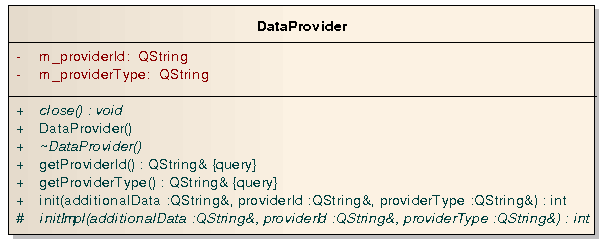
\includegraphics[width=0.7\textwidth]{img/provider.png}
\end{figure}

Należy również nadmienić, że konieczne było również dostarczenie
odpowiedniego mechanizmu rejestracji definiowanych obiektów
w~fabryce. Istotne jest, aby umożliwić programiście rejestrację nowego
typu faktycznego obiektu bez konieczności ingerencji w~inne pliki
źródłowe. W~celu ułatwienia tego procesu zostało opracowane makro,
które dzięki wykorzystaniu szablonów dokonuje automatycznej
rejestracji nowego typu faktycznego obiektu w~fabryce. Dzięki jego
wykorzystaniu programista podczas dodawania nowego dostawcy danych,
musi zapewnić jedynie deklarację oraz definicję nowego typu. Warto
zauważyć, że sposób implementacji tego makra pozwala na umieszczenie
definicji nowego typu w~pliku nagłówkowym, który jest włączany do
wielu jednostek translacji i nie powoduje to błędów kompilacji ani
błędów funkcjonowania procesu rejestracji.

\vspace{0.5cm}
\begin{minipage}{\textwidth}
\begin{lstlisting}[language=c++, caption=Definicja dostawcy danych, linewidth=10cm]
DATA_PROVIDER(NazwaTypu, NazwaRejestrowana)
{
  //deklaracja metod
}
\end{lstlisting}
\end{minipage}
\vspace{0.5cm}

W~ramach tej grupy obiektów dostarczono również referencyjną
implementację dostawcy o~nazwie typu {\em DefaultTcpProvider}. Stanowi
on implementację omówionego wcześniej protokółu
komunikacyjnego. W~celu zapewnienia lepszej wydajności logika
funkcjonowania tego dostawcy została przeniesiona do osobnego wątku
programu. Aby zapewnić elastyczności wykorzystania tego obiektu
możliwe jest zarówno definiowanie z~poziomu pliku konfiguracyjnego
adresu IP i~portu wykorzystywanego przez ten obiekt, jak i~wskazanie
pliku zawierającego klucz prywatny.

\subsubsection[Grupa obiektów konsumentów danych][Grupa obiektów
konsumentów danych]{Grupa obiektów konsumentów danych}

Grupa obiektów konsumentów danych posiada analogiczną budowę jak grupa
producentów danych. Zapewnia ona fabrykę konsumentów danych
i~generyczny interfejs konsumenta. Interfejs konsumenta danych jest
analogiczny jak dla dostawcy. Rejestracja obiektów w~fabryce odbywa
się również przy użyciu analogicznego makra. W~ramach tej grupy
obiektów dostarczono implementację dwóch konsumentów danych. Pierwszy
z~nich, o~nazwie typu {\em ToScreenPrinter}, spełnia jedynie funkcję
kontrolną. Wszystkie dane, które do niego trafią, są natychmiast
wypisywane w~dzienniku wykonania programu. Dostawca typu {\em
  ToIcingaWriter} odpowiedzialny jest natomiast za przekazywanie
wszystkich danych do pliku komend zewnętrznych systemu {\em Icinga}. Możliwa
jest zmiana ścieżki pliku komend zewnętrznych systemu {\em Icinga} poprzez
plik konfiguracyjny.

\subsubsection[Grupa obiektów filtracji][Grupa obiektów
filtracji]{Grupa obiektów filtracji}

Grupa obiektów filtracji pozwala na kontrolę danych otrzymywanych od
klienta, a~także na pobieranie informacji o~danym
kliencie. Podstawowym elementem tej tej grupy jest fizyczne
odwzorowanie bytu klienta w odpowiednią klasę. Pozwala to na
uzyskiwanie przez inne moduły w prosty sposób wszystkich niezbędnych
informacji na temat obsługiwanego klienta. Każdy klient posiada
zdefiniowany w~pliku konfiguracyjnym zbiór urządzeń i~usług, o~których
informacje może przesyłać. Obiekty z~tej grupy, które są
odpowiedzialne za kontrolę odbieranych danych, pobierają z~analizatora
składniowego wspomniane zbiory i~dokonują kontroli każdego wpisu
dziennika otrzymanego od klienta. Jeśli klient nadesłał dane
dotyczące urządzenia lub usługi, do których nie ma on uprawnień, nie
będzie możliwe przekazanie ich do konsumentów.

\subsubsection[Grupa obiektów kanału komunikacyjnego][Grupa obiektów
kanału komunikacyjnego]{Grupa obiektów kanału komunikacyjnego}

Grupa obiektów kanału komunikacyjnego odpowiedzialna jest za
niezawodne przekazanie danych od dostawcy danych do konsumentów według
reguł zdefiniowanych w~pliku konfiguracyjnym. Zapewnienie
niezawodności zostało osiągnięte poprzez implementację bufora kołowego
wewnątrz pliku. Każdy dostawca danych posiada swój plik bufora. Na
początku tego pliku zapisane są położenia miejsca przeznaczonego do
czytania oraz miejsca przeznaczonego do pisania. Dane, które logicznie
znajdują się pomiędzy miejscem do czytania, a~miejscem do pisania, są
to dane, które zostały odebrane od klienta, lecz nie zostały jeszcze
dostarczone do konsumentów. Pomyślnie zweryfikowana przez obiekty
filtrujące porcja danych przekazywana jest z~użyciem kanału
komunikacyjnego do konsumentów danych. Operacja ta odbywa się w~dwóch
etapach. Pierwszy etap dokonuje zapisu danych do pliku bufora. Jeśli
aktualnie nie ma żadnych danych oczekujących na przetworzenie przez
konsumentów, nowa porcja danych jest niezwłocznie dostarczana do
odpowiednich obiektów. Jeśli istnieją porcje danych, które oczekują na
zapisanie, dane zostaną zapisane do pliku i~dostarczone po danych,
które nadeszły przed nimi. Należy zwrócić uwagę, że dane zapisywane są
na dysku tylko raz, niezależnie od liczby konsumentów, do których
powinny one zostać dostarczone. Ponadto dostawca danych uzyskuje
potwierdzenie zapisania danych po zakończeniu pierwszego etapu ich
obsługi, czyli już po zapisaniu do pliku bufora. Oznacza to, że dostawcy
danych są w~znacznym stopniu niezależni od konsumentów danych. Pozwala
to skrócić do minimum czas oczekiwania klienta mobilnego pomiędzy
wysłaniem danych, a~uzyskaniem potwierdzenia o~ich przetworzeniu.

\subsubsection[Grupa obiektów zarządzających][Grupa obiektów
zarządzających]{Grupa obiektów zarządzających}

Głównym przedstawicielem grupy obiektów zarządzających jest klasa
główna programu. Program został napisany zgodnie z~metodyką obiektową,
zatem cała logika wykonania programu została również zamknięta
w~klasie, co uprościło funkcję główną programu do minimum. Klasa ta
odpowiedzialna jest za przebieg całości programu. Pierwszą operacją
wykonywaną przez tę klasę jest odnalezienie pliku konfiguracyjnego
i~zlecenie jego wczytania przez parser konfiguracji. Na podstawie
informacji uzyskanych w~wyniku analizy pliku konfiguracyjnego klasa
główna programu pobiera z~odpowiednich fabryk wszystkie obiekty
producentów oraz konsumentów zdefiniowanych w~pliku
konfiguracyjnym. Po uzyskaniu obiektów następuje ich inicjalizacja na
podstawie danych wczytanych z pliku konfiguracyjnego. Klasa ta jest
również odpowiedzialna za prawidłową deinicjalizację oraz destrukcję
wszystkich obiektów. Ponadto należy zauważyć, że omawiany program
funkcjonuje jako serwis systemowy, zatem konieczne jest również
wykonanie w~tej klasie wszystkich czynności zalecanych przy
uruchamianiu takich serwisów. Całość programu została napisane zgodnie
z~paradygmatem zdarzeniowym. Oznacza to, że po wykonaniu inicjalizacji,
program zawiesza swoje wykonanie do czasu otrzymania jakiegoś
zdarzenia, na które powinien on zareagować. Użycie biblioteki Qt w
znaczny sposób uprościło oczekiwanie na zdarzenia dzięki możliwości
użycia pętli zdarzeń z tej biblioteki.

\section[Moduł kryptograficzny][Moduł kryptograficzny]{Moduł kryptograficzny}

Moduł ten dostarcza pozostałym elementom programu implementacji
algorytmów kryptograficznych. Dostępne są generyczne interfejsy do
następujących schematów algorytmów:

\begin{itemize}
\item szyfrowanie symetryczne,
\item szyfrowanie asymetryczne,
\item funkcja skrótu,
\item podpis cyfrowy.
\end{itemize}

\begin{figure}[htbp]
  \centering
  \caption{Interfejsy algorytmów kryptograficznych.}
  \label{fig:cryptoInterface}
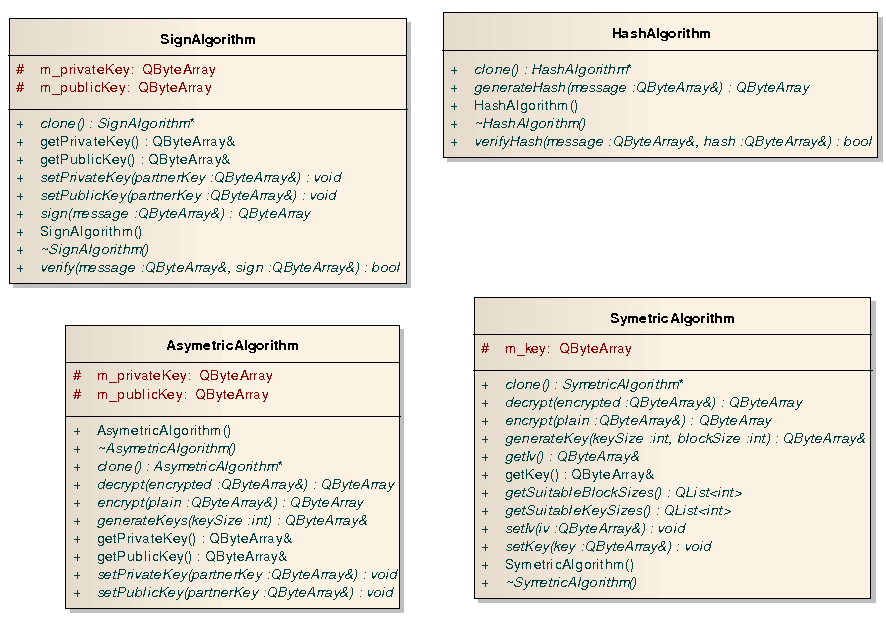
\includegraphics[width=1\textwidth]{img/crypto.png}
\end{figure}

Definicje wszystkich interfejsów zostały przedstawione na
rys.~\ref{fig:cryptoInterface}. Dostarczanie implementacji danego
schematu kryptograficznego odbywa się w~sposób analogiczny do
dostarczania implementacji dostawców danych. Wszystkie implementacje
algorytmów zostają zarejestrowane w~fabryce kryptograficznej, która
umożliwia uzyskiwanie obiektu o~typie określanym na podstawie danych,
na przykład odebranych od klienta.

% biblio do CBC i AESA
W~ramach tej pracy dostarczono kilku algorytmów, które były konieczne
do zaimplementowania protokołu komunikacyjnego. Jako algorytm
symetryczny dostarczona została implementacja algorytmu AES
pracującego w~trybie wiązania bloków zaszyfrowanych. Omawiany tryb
pracy algorytmu powoduje powstanie zależności pomiędzy kolejnymi
blokami. Oznacza to, że manipulacja jednym blokiem powoduje zmiany
wartości odszyfrowanych w~tym bloku i~każdym następnym. Zastosowanie
tego trybu w~implementowanym protokole komunikacyjnym pozwala na
zagwarantowanie, że sekwencja wiadomości otrzymywanych od klienta nie
została zmieniona\footnote{Samo wykorzystanie trybu CBC nie daje
  gwarancji ale w protokole komunikacyjnym użyto również
  funkcji skrótu, przez co możliwe jest jej udzielenie.}. Protokół
komunikacyjny wymagał również dostarczenia asymetrycznego algorytmu
RSA. W~module zdefiniowano ponadto klasę implementującą generyczny
interfejs funkcji skrótu, która dostarcza funkcjonalności algorytmu
SHA-2 o~długości skrótu 256 bitów. Jeden z~etapów protokołu
komunikacyjnego wymagał również dostarczenia algorytmu podpisu
cyfrowego opartego na algorytmie RSA.

Do implementacji wszystkich algorytmów została wykorzystana biblioteka
Crypto++. Jest to popularna biblioteka o~otwartych źródłach, napisana
w~języku~C++, która w~obiektowy sposób udostępnia algorytmy
kryptograficzne.

\section[Moduł uwierzytelnienia][Moduł uwierzytelnienia klienta]{Moduł uwierzytelnienia klienta}

Moduł posiada architekturę typową dla modułów usługowych. Głównym
elementem jest klasa implementująca wzorzec fabryki oraz generyczny
interfejs pozwalający na wykorzystywanie obiektów uzyskanych
z~fabryki.

Interfejs zdefiniowany dla algorytmów uwierzytelnienia został
zaprojektowany z~wykorzystaniem mechanizmu sygnałów i~slotów
z~biblioteki Qt. Użycie tego mechanizmu pozwala na znacznie
wydajniejsze wykorzystanie zasobów. Przykładem takiej optymalizacji
może być czas, gdy klient przetwarza żądanie związanie
z~uwierzytelnieniem.  Wątek serwera nie musi być wtedy bezczynny, lecz
może przetwarzać żądania pochodzące od innych klientów. Definicja
interfejsu pozwala również na przekazanie do niego dodatkowych
ustawień pochodzących z~pliku konfiguracyjnego. Każdy algorytm
uwierzytelnienia powinien po zakończeniu sukcesem lub porażką procesu
uwierzytelnienia klienta wykonać emisję sygnału z~interfejsu algorytmu
wraz z~rezultatem procesu autoryzacji. Ponieważ z~punktu widzenia
protokołu istotne jest przekazanie danych autoryzacyjnych jako
informacji o~akceptacji algorytmu uwierzytelnienia, konieczne jest, aby
każdy algorytm przesłał co najmniej jedną wiadomość do klienta.

Zapewnienie niezależności implementacji algorytmów uwierzytelnienia od
wykorzystywanej aktualnie metody komunikacji wymagało zdefiniowania
generycznego interfejsu komunikacyjnego, który może być wykorzystywany
przez implementacje poszczególnych algorytmów. Implementacja tego
interfejsu powinna być dostarczona przez moduł, który jest aktualnie
wykorzystywany w~programie do komunikacji z~klientem.

\begin{figure}[htpb]
  \centering
  \caption{Przykładowy przebieg procesu uwierzytelnienia.}
  \label{fig:sekwencjaAuth}
  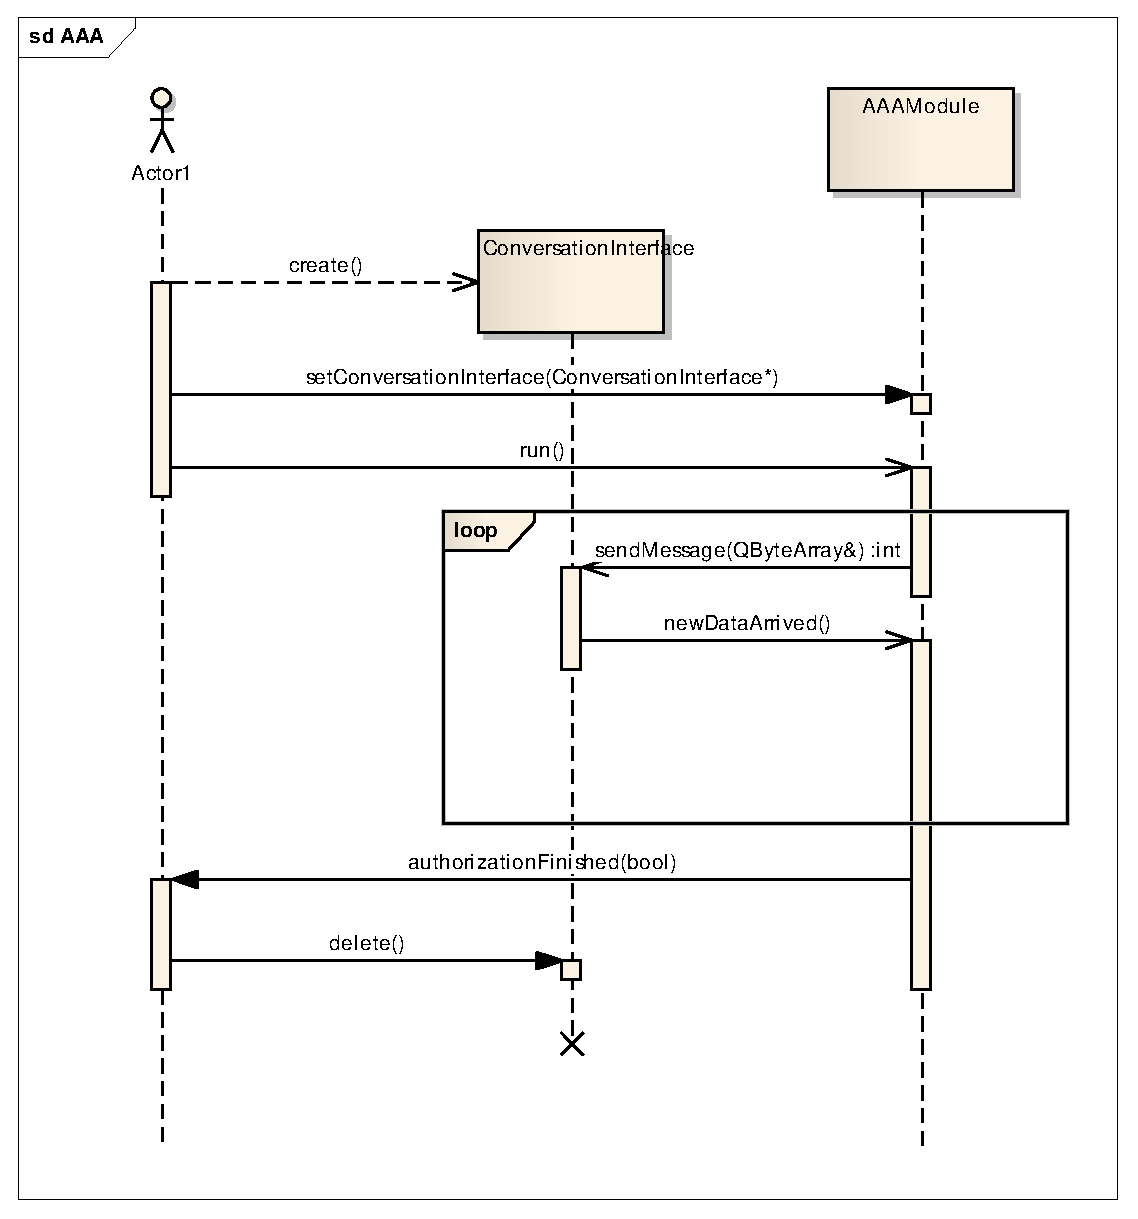
\includegraphics[width=1\textwidth]{img/aaa}
\end{figure}

Przykładowy przebieg procesu uwierzytelnienia został przedstawiony na
rys.~\ref{fig:sekwencjaAuth}. Proces ten rozpoczyna się od ustawienia
aktualnie wykorzystywanego interfejsu komunikacyjnego. Następnie
wykonywane jest rozpoczęcie procesu uwierzytelnienia. W ramach tego
procesu moduł uwierzytelnienia może komunikować się z klientem poprzez
otrzymany wcześniej obiekt. Po zakończeniu procesu autoryzacji
emitowany jest odpowiedni sygnał informujący pozostałe komponenty o
rezultacie uwierzytelnienia.

W~ramach pracy został zaimplementowany również przykładowy moduł
uwierzytelnienia klienta. Nosi on nazwie: {\em LoginPass}. Jest to
prosta metoda uwierzytelnienia oparta na pobraniu od klienta loginu
oraz hasła i~porównanie go z~danymi dostarczonymi w~pliku
konfiguracyjnym. Każdy klient posiada w~pliku konfiguracyjnym listę
dostępnych dla niego algorytmów uwierzytelnienia wraz z~danymi, jakie
powinny być przekazane, aby zapewnić pozytywne wykonanie
procesu. Należy zwrócić uwagę, że zaimplementowany algorytmy
uwierzytelnienia stanowi jedynie przykład, w jaki sposób powinno się
definiować algorytmy w opracowanym dodatku. Ich wykorzystanie w
systemie produkcyjnym zależy od bezpieczeństwa serwera, na którym
znajduje się program NSCAv2. Należy być świadomym, że wszystkie hasła
oraz nazwy użytkowników przechowywane są jawnym tekstem w~pliku
konfiguracyjnym\footnote{Sposób przechowywania loginu oraz hasła na
  urządzeniu mobilnym jest uzależnione od konkretnej implementacji
  aplikacji IcingaMini.}. Nie stanowi to oczywiście zagrożenia jeśli
do serwera monitorującego dostęp mają jedynie uprzywilejowane
osoby. Należy przypomnieć, że na serwerze znajdują się również klucze
prywatne RSA, więc zawsze należy zwrócić szczególną uwagę, na
bezpieczeństwo serwera.

\section[Moduł TCP][Moduł komunikacji z wykorzystaniem TCP]{Moduł komunikacji z wykorzystaniem TCP}

Moduł ten zawiera implementację protokołu komunikacyjnego opisanego
w~rozdziale~\ref{sec:ProtKom}. Inicjacja każdej z~warstw protokołu
została zaimplementowana w~dedykowanej klasie lub jeśli proces
inicjacji złożony był z~kilku rozdzielnych logicznie elementów, każdy
element został zaimplementowany w~osobnej klasie. W~celu umożliwienia
każdej z~warstw protokołu korzystanie z~usług warstw niższych,
w~sposób generyczny wykorzystany został wzorzec dekoratora.

Aby wykorzystać wzorzec dekoratora (patrz rys.~\ref{fig:Dekorator}),
zdefiniowano generyczny interfejs pozwalający na odczytanie oraz
zapisanie komunikatu niezależnie od liczby warstw znajdujących się
poniżej. Klasą prostą w~tym przypadku jest prosta klasa opakowująca
gniazdo TCP z~biblioteki Qt. Klasami dekorującymi są klasy
odpowiadające za kolejne czynności w wyższych warstwach
protokołu. Klasy te są odpowiedzialne za formowanie wiadomości,
szyfrowanie oraz obliczanie i~kontrolę jej skrótu. Ponieważ kolejność
czynności wykonywanych w~trakcie budowania wiadomości jest istotna,
zastosowano enkapsuowane budowanie wiadomości. Każda klasa dekoratora
posiada tylko jedno wskazanie do obiektu, który znajduje się o~poziom
niżej w hierarchii. Użytkownik zapisuje wiadomość, używając klasy
z~najwyższej warstwy. Obiekt ten dokonuje przekształcenia wiadomości
zgodnie ze swoim algorytmem, a~następnie wywołuje tę samą metodę na
rzecz obiektu znajdującego się o~jeden niżej w~hierarchii niż ona
sama, przekazując przekształconą wiadomość jako parametr wywołania.

%diagram z tymi klasami

\begin{figure}[htpb]
  \centering
  \caption{Diagram klas wykorzystujących wzorzec dekoratora.}
  \label{fig:Dekorator}
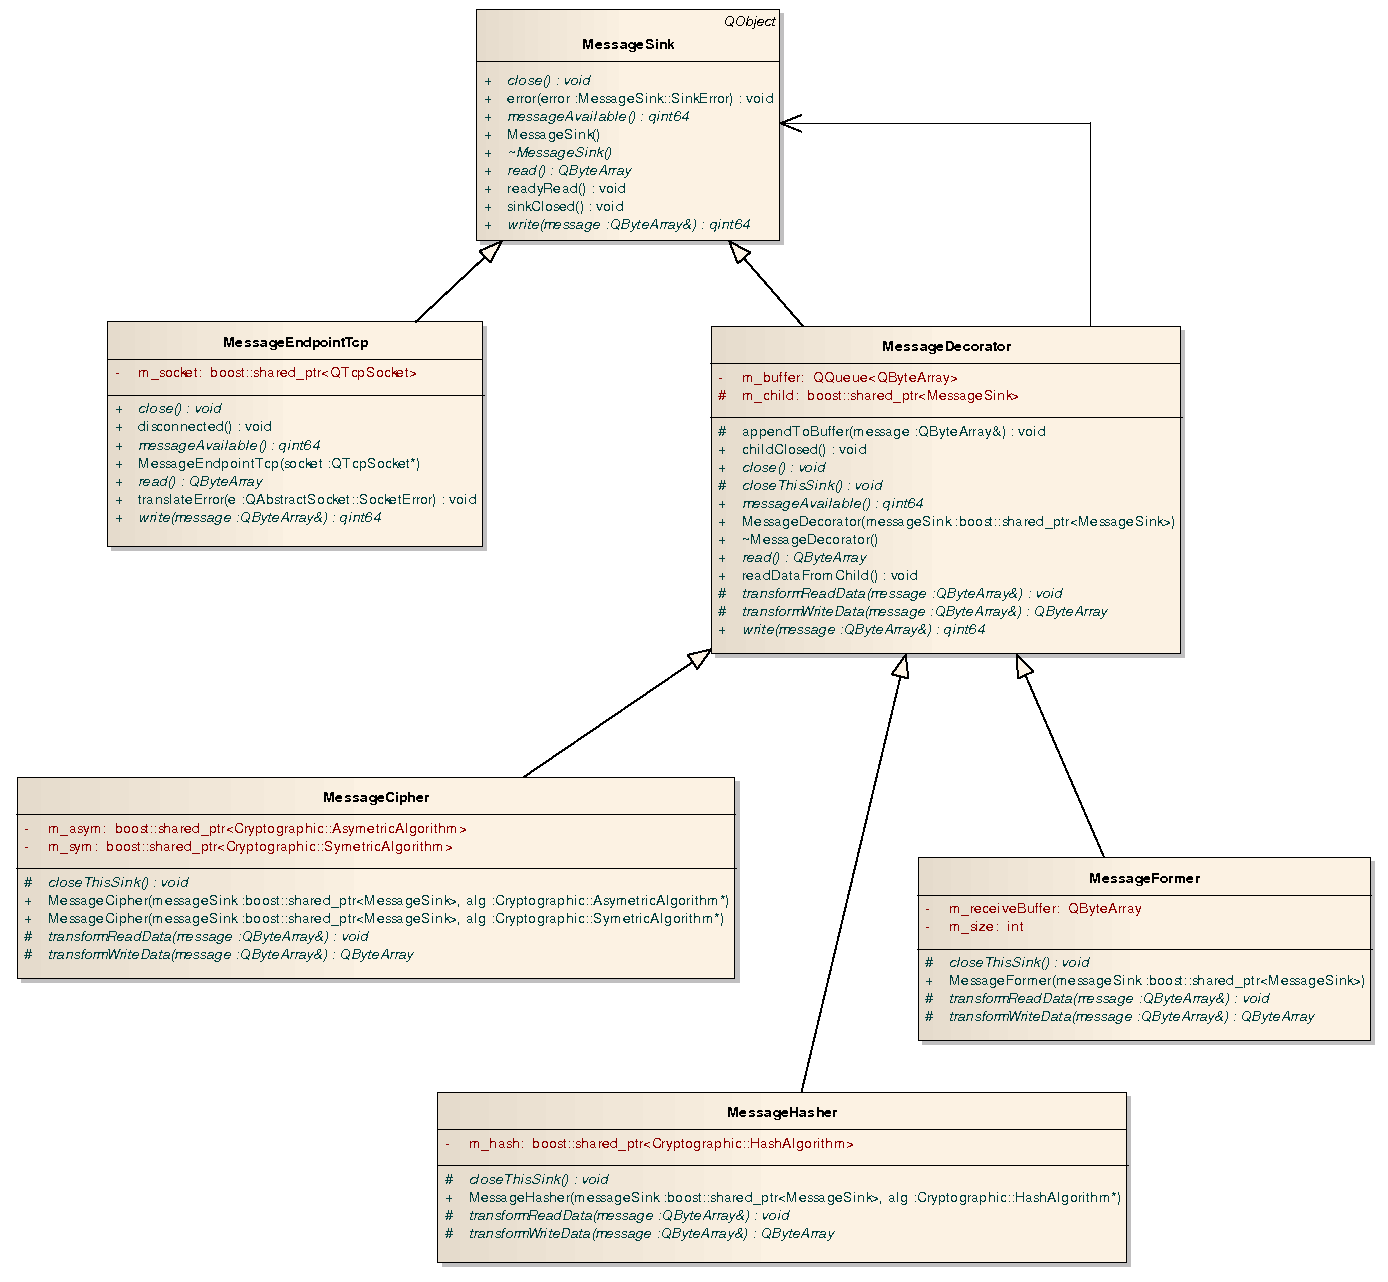
\includegraphics[width=1\textwidth]{img/dekorator.png}
\end{figure}

Wykorzystanie wzorca dekoratora pozwoli w~przyszłości na łatwą
modyfikację protokołu komunikacyjnego, np. poprzez dodatkową
warstwę. Ponadto wprowadzenie jednolitego interfejsu pozwoliło na
zachowanie prostoty i~jednolitości implementacji poszczególnych warstw
protokołu komunikacyjnego.

Moduł ten został zaimplementowaniu przy użyciu licznych mechanizmów
z~biblioteki Qt. Przede wszystkim wykorzystany został moduł sieciowy
wspomnianej biblioteki. Dzięki jego użyciu uzyskano dostęp do
generycznej implementacji serwera TCP, a~także gniazd. Szkielet
aplikacji Qt pozwolił na wygodną implementację asynchronicznej
komunikacji z~użyciem gniazd TCP przy pomocy standardowego dla tego
szkieletu mechanizmu sygnałów i~slotów. Dzięki temu uzyskano
przejrzysty i~wydajny kod, który pozwala na obsługę wielu klientów
w~jednym wątku.

\section[Moduł logowania][Moduł logowania]{Moduł logowania}

Omawiany dodatek wykonywany jest bez interakcji
z~użytkownikiem. Funkcjonuje on jako serwis systemowy. Docelowo będzie
wykonywany na serwerze, poza sesją jakiegokolwiek
użytkownika. W~trakcie wykonania programu mogą się zdarzyć sytuacje
wymagające poinformowania użytkownika o~ich wystąpieniu. Znaczna część
z~tych informacji stanowi jedynie zapis wykonania programu, jednak
mogą występować również informacje o sytuacjach krytycznych, o których
użytkownik musi zostać powiadomiony. Konieczne było zatem dostarczenie
możliwości przekazywania takich informacji z~wielu modułów do jednego,
wspólnego miejsca, które stanowi dziennik wykonania serwisu.

Każdy moduł posiada możliwość przekazywania użytkownikowi wiadomości
o~różnym priorytecie. Dozwolone są następujące priorytety:

\begin{description}
\item[FATAL] --- najwyższy priorytet, wiadomość zawiera komunikat
  o~błędzie, który uniemożliwia dalsze wykonanie programu.
\item[ERROR] --- komunikat zawiera informacje o~błędzie, który
  uniemożliwia wykonanie pewnej ścieżki programu.
\item[WARNING] --- komunikat zawiera ostrzeżenie o~nietypowej sytuacji.
\item[DEBUG] --- komunikat zawiera treść pomocną podczas wyszukiwania błędów.
\item[INFO] --- komunikat zawiera jedynie treści informacyjne.
\end{description}

Podczas kompilacji ustalany jest minimalny priorytet wiadomości, które
mają być przekazywane użytkownikowi. Wszystkie wiadomości
o~priorytecie niższym niż ustalony nie zostaną zapisane. Ponadto
dzięki użyciu mechanizmów opartych o~szablony wszystkie komunikaty
o~priorytecie niższym zostaną rozwinięte do wywołania funkcji
pustej. Wywołanie takie zostanie z bardzo dużym prawdopodobieństwem
zoptymalizowane przez kompilator.

Przekazanie użytkownikowi treści komunikatu w~wielu sytuacjach może
nieść zbyt mało informacji. Aby umożliwić przekazanie dodatkowych
informacji bez konieczności pisania nadmiernej liczby komend przy
każdym komunikacie, opracowana została makrodefinicja, która do
każdego komunikatu dołączy aktualny stempel czasu, nazwę pliku,
w~którym znajduje się komunikat, a~także nazwę funkcji oraz numer
linii. Ponadto komunikat nie musi się składać jedynie z~tekstu, lecz
można go formować w~taki sam sposób jak pisać do strumienia.

\vspace{0.5cm}
\begin{minipage}{\textwidth}
  \begin{lstlisting}[language=c++, breaklines=true,
    linewidth=0.99\textwidth, caption=Przykładowe wypisanie
    komunikatu.]

LOG_ENTRY(MyLogger::DEBUG, "komunikat"<<123);

\end{lstlisting}
\end{minipage}
\vspace{0.5cm}

\vspace{0.5cm}
\begin{minipage}{\textwidth}
\begin{lstlisting}[linewidth=0.99\textwidth, caption=Format komunikatu przekazywanego użytkownikowi.]

[stempel czasu][poziom][plik][funkcja][linia]:komunikat123

\end{lstlisting}
\end{minipage}
\vspace{0.5cm}

Ponieważ demon nie jest przypisany do żadnego
z~terminali\footnote{Proces przekształcenia w serwis systemowy zakłada
  zamknięcie deskryptorów standardowego wejścia, wyjścia oraz wyjścia
  błędów.}, nie ma możliwości przekazywania wiadomości na standardowe
wyjście lub wyjście błędów. Konieczne jest zatem utworzenie pliku, do
którego zapisywane będą komunikaty. Należy zwrócić uwagę, że program
jako serwis systemowy uruchomiony będzie ze znacznie ograniczonymi
prawami, aby podnieść poziom bezpieczeństwa serwera. W~związku
z~powyższym jedynym miejscem, co do którego można założyć, że program
będzie miał dostęp, jest katalog plików tymczasowych. Każde
uruchomienie programu powoduje zatem utworzenie w~tym katalogu pliku
składającego się z~nazwy programu oraz stempla czasu zawierającego
czas jego uruchomienia.
